\subsection{Bring everything together}
\href{https://docs.godotengine.org/en/stable/getting_started/first_2d_game/05.the_main_game_scene.html}{\color{blue}The main game scene}.
Add main scene containing player and mob scenes. Additionally, this scene controlls the flow of the game by handling timers.
Create new scene by adding a \textit{Node} called \textbf{Main}. Then click on the \textbf{Instance} button (see cursor
on the image) and select \textit{player.tscn}.
\begin{figure}[H]
    \centering
    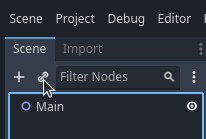
\includegraphics[scale=0.5]{main-scene.png}
    \caption{workspace after enemy creation}
    \label{fig:main-scene}
\end{figure}
Add three Timer objects to \textit{Main} and name them and set \textit{Wait Time} property as follows:
\begin{itemize}
    \item MobTimer - control mobs spawn: 0.5
    \item ScoreTimer - increment score by seconds: 1
    \item StartTimer - delay before starting: 2
\end{itemize}
Additionally, create a \textit{Marker2D} for the starting position of the player and set its \textit{Position} property
to 240, 450.
\subsubsection{Spawning mobs}
Enemies should be created randomly on the edge of the screen. To achieve this, add a \textit{Path2D} node and call it
\textbf{MobPath} as child of \textbf{Main}. Select the 4 corners of the screen to setup the path of the curve used
for spawning enemy objects. Finally, a \textit{PathFollow2D} node needs to be added as a child of \textbf{MobPath},
name it \textbf{MobSpawnLocation}. The scene is expected to look as below with the created curve:
\begin{figure}[H]
    \centering
    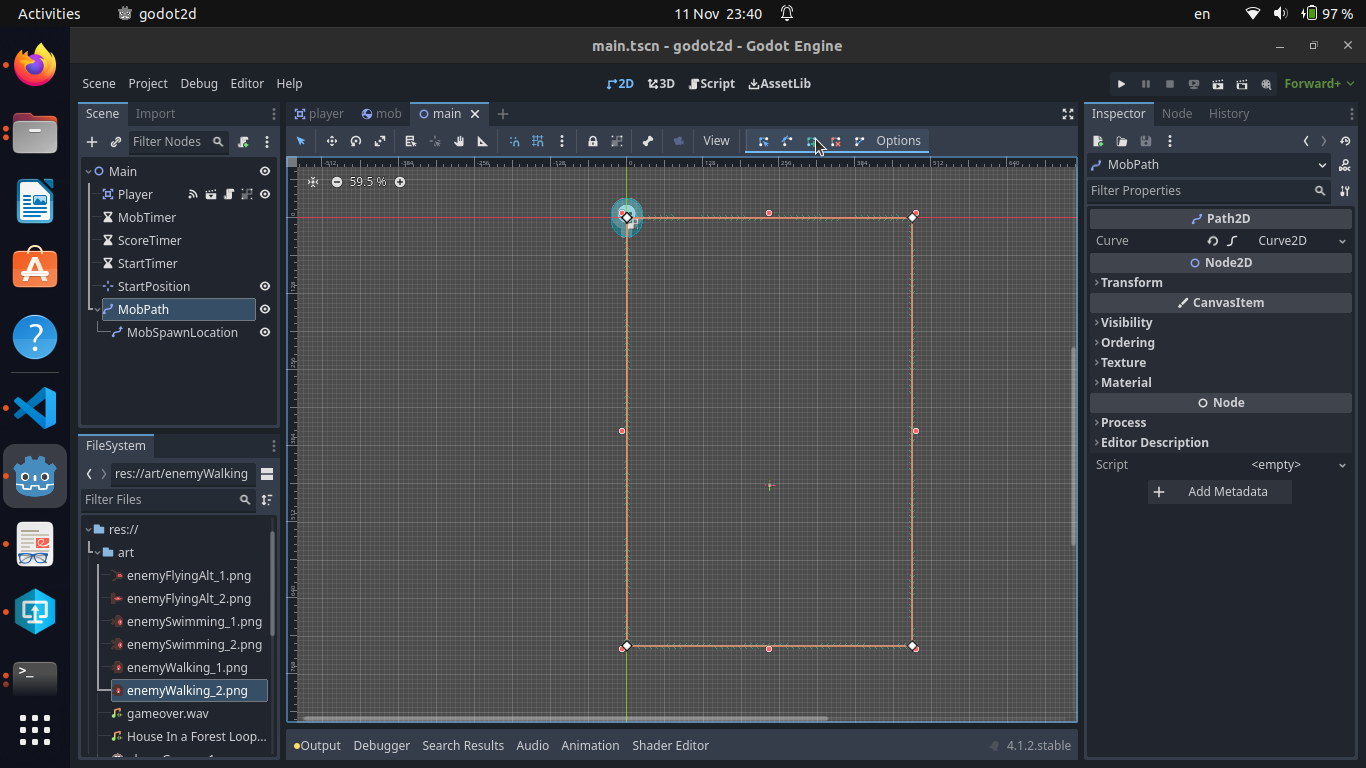
\includegraphics[width=\textwidth]{mobpath.png}
    \caption{mob path}
    \label{fig:mobpath}
\end{figure}
Add a script to the main scene with the following content:
\begin{verbatim}
    extends Node

    @export var mob_scene: PackedScene
    var score
    
    # Called when the node enters the scene tree for the first time.
    func _ready():
        pass #new_game()
    
    
    # Called every frame. 'delta' is the elapsed time since the previous frame.
    func _process(delta):
        pass
    
    
    func game_over():
        $ScoreTimer.stop()
        $MobTimer.stop()
        
    func new_game():
        score = 0
        $Player.start($StartPosition.position)
        $StartTimer.start()
    
    func _on_start_timer_timeout():
        $MobTimer.start()
        $ScoreTimer.start()
    
    func _on_score_timer_timeout():
        score += 1
    
    func _on_mob_timer_timeout():
        # Create a new instance of the Mob scene.
        var mob = mob_scene.instantiate()
    
        # Choose a random location on Path2D.
        var mob_spawn_location = get_node("MobPath/MobSpawnLocation")
        mob_spawn_location.progress_ratio = randf()
    
        # Set the mob's direction perpendicular to the path direction.
        var direction = mob_spawn_location.rotation + PI / 2
    
        # Set the mob's position to a random location.
        mob.position = mob_spawn_location.position
    
        # Add some randomness to the direction.
        direction += randf_range(-PI / 4, PI / 4)
        mob.rotation = direction
    
        # Choose the velocity for the mob.
        var velocity = Vector2(randf_range(150.0, 250.0), 0.0)
        mob.linear_velocity = velocity.rotated(direction)
    
        # Spawn the mob by adding it to the Main scene.
        add_child(mob)
\end{verbatim}
The \textit{Main} node needs to be able to access variables from \textit{Mob} scene. For this, the 
\textit{Mob Scene} {$<$}empty{$>$} button in the \textit{Inspector} tab and load \textit{mob.tscn} in the pop-up window.
\begin{figure}[H]
    \centering
    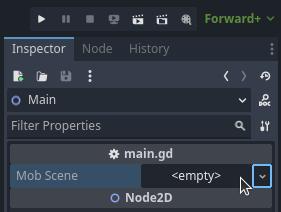
\includegraphics[scale=0.5]{mob-scene-variables.png}
    \caption{mob scene variables}
    \label{fig:mob-scene-variables}
\end{figure}
Sort out signals:
\begin{itemize}
    \item Connect the \textit{hit} signal of the player scene with a receiver method called \textbf{game\_over}.
    \item Connect \textit{timeout()} signal of each Timer nodes to the main script.
\end{itemize}
Now, pressing F5 should run the game with a player character disappearing when being hit by an enemy.

\subsection{Version control of final steps}
Having done all the steps above, commit changes to the \textit{dev1.0} stream, the version control system shows the below
picture: \hfill \break
\begin{figure}[H]
    \centering
    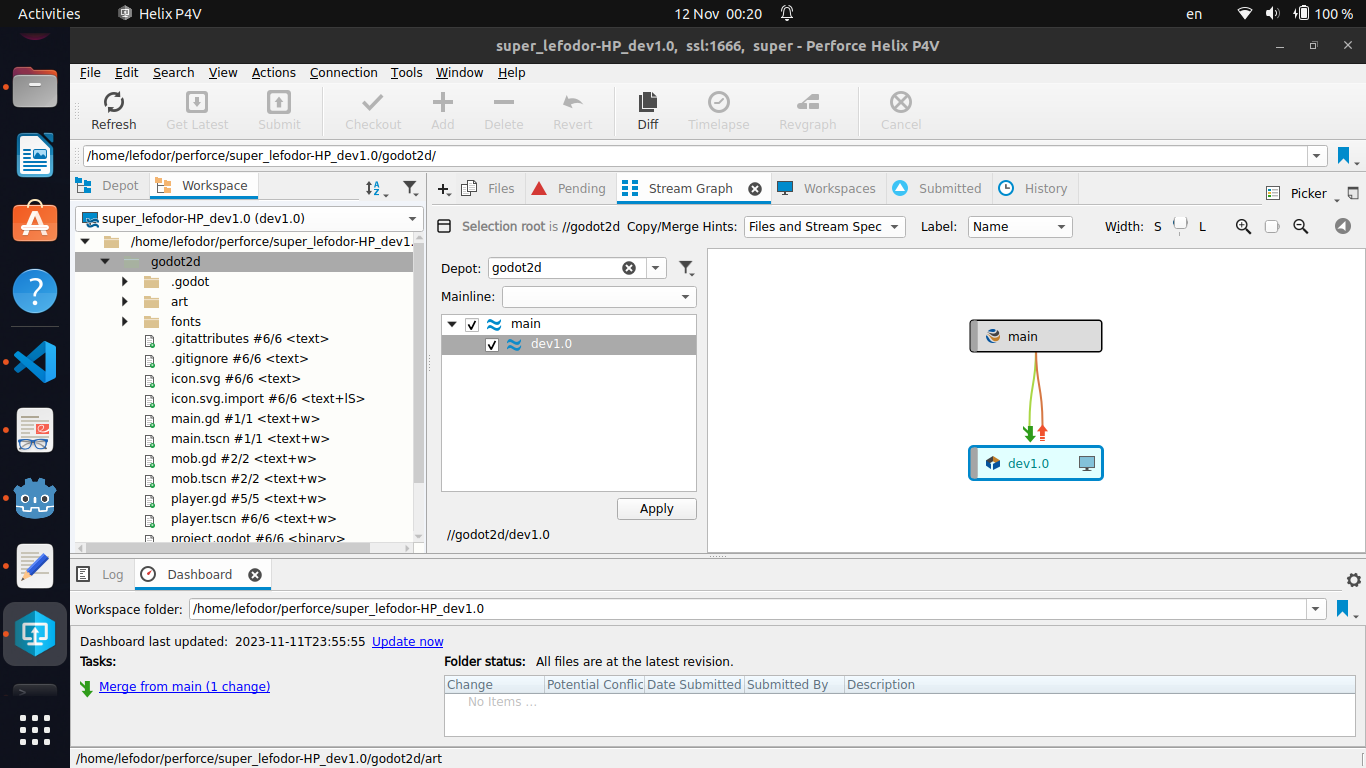
\includegraphics[width=\textwidth]{copy-merge-main.png}
    %\setlength{\belowcaptionskip}{-50pt}
    \caption{copy merge main}
    \label{fig:copy-merge-main}
\end{figure}
The orange arrow means there is a need to merge changes from the \textit{main} stream and only after this becomes possible 
to copy files from the development stream back to main. \hfill \break
Proceeding with the merge (downstream synchronization from more stable (main) stream towards less stable (development)
stream), the below conflict is shown:
\begin{figure}[H]
    \centering
    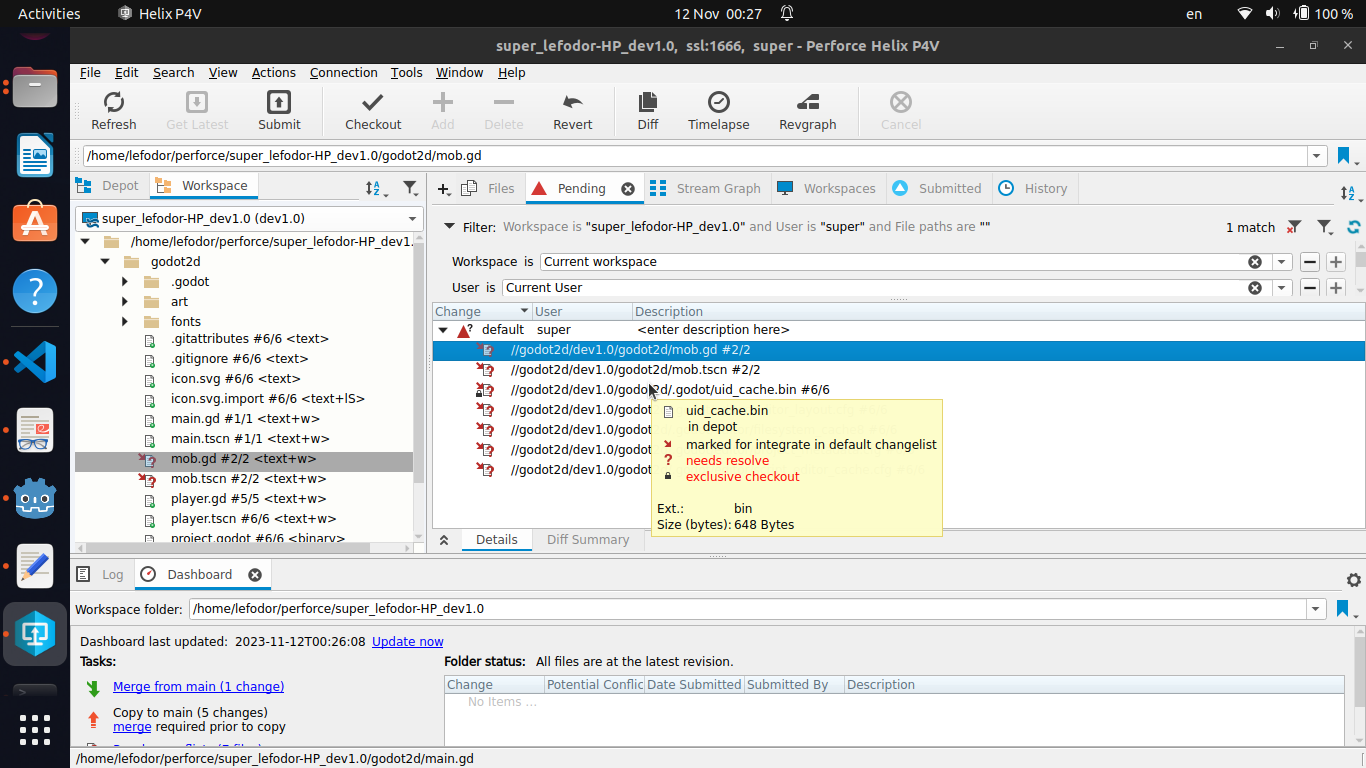
\includegraphics[width=\textwidth]{show-main-dev-conflict.png}
    \caption{show main dev conflict}
    \label{fig:show-main-dev-conflict}
\end{figure}
The conflicts are needed to be resolved manually to make sure the correct version is retained. The \textit{Resolve} pop-up
window shows the possibilities to Accept Source/Target/Merged or Run Merge Tool. For all conflicts, the 'Accept Target'
option was selected as only the \textit{dev1.0} stream was updated during development process, different versions in the 
\textit{main} stream may only occur due to autosave method of the game engine. If not only one developer works on the project
then the merge/copy history has to be checked and select the proper resolve method accordingly.

\begin{figure}[H]
    \centering
    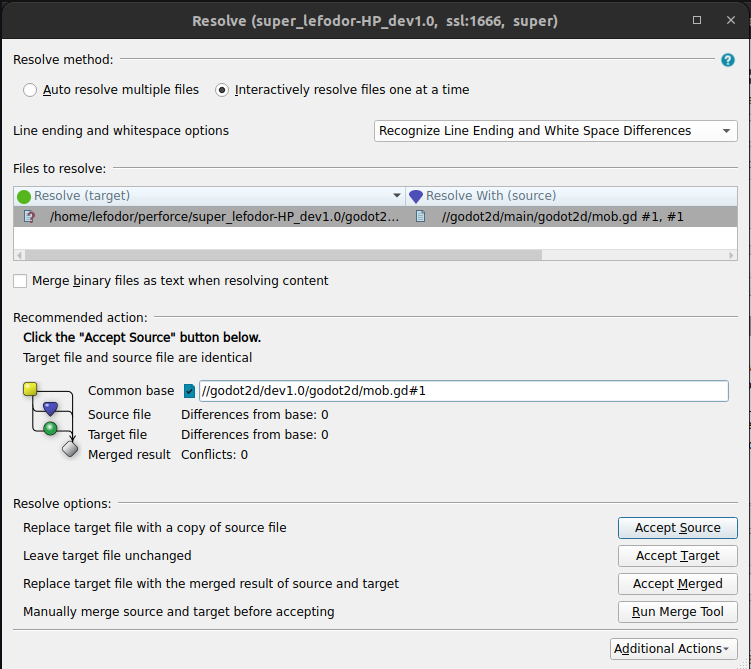
\includegraphics[scale=0.5]{resolve-main-dev-conflict.png}
    \setlength{\belowcaptionskip}{-10pt}
    %\setlength{\intextsep}{5pt}
    \caption{resolve main dev conflict}
    \label{fig:resolve-main-dev-conflict}
\end{figure}

After resolving the conflicts, the copy method from the \textit{dev1.0} stream is possible (green arrow).
\begin{figure}[H]
    \centering
    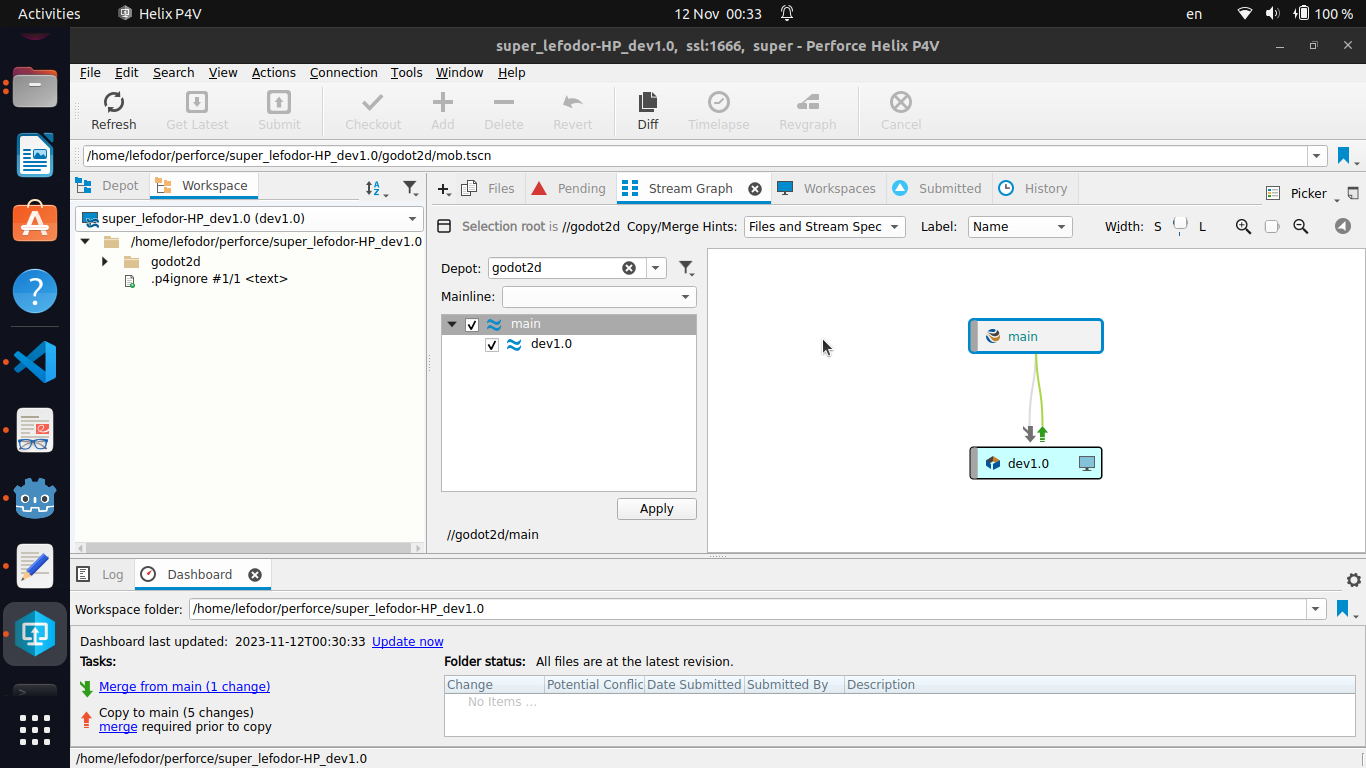
\includegraphics[width=\textwidth]{after-merge-conflicts-resolved.png}
    \caption{after merge conflicts resolved}
    \label{fig:after-merge-conflicts-resolved}
\end{figure}
As a last step, we can observe the change history for both \textit{main} and \textit{dev1.0} streams 
\begin{figure}[H]
    \centering
    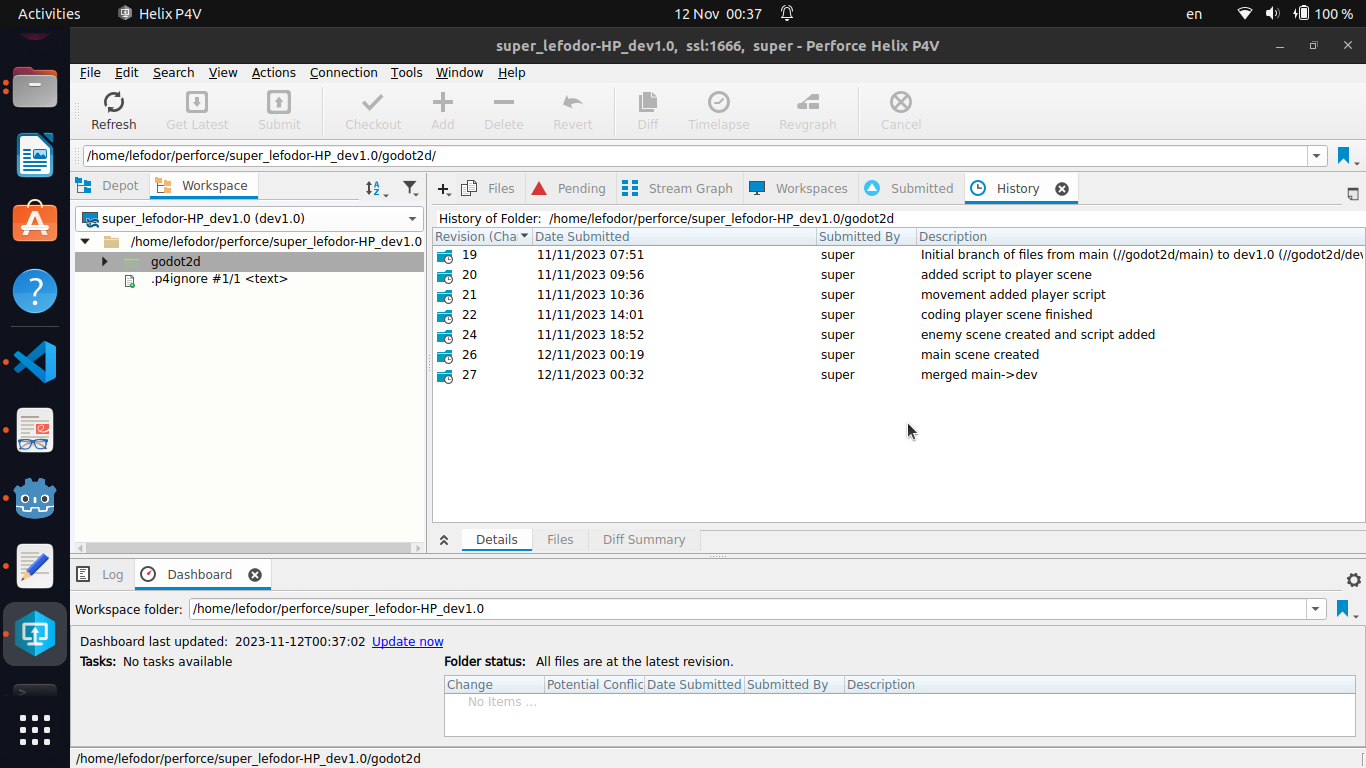
\includegraphics[width=\textwidth]{final-dev1-history.png}
    \caption{final dev1 history}
    \label{fig:final-dev1-history}
\end{figure}

\begin{figure}[H]
    \centering
    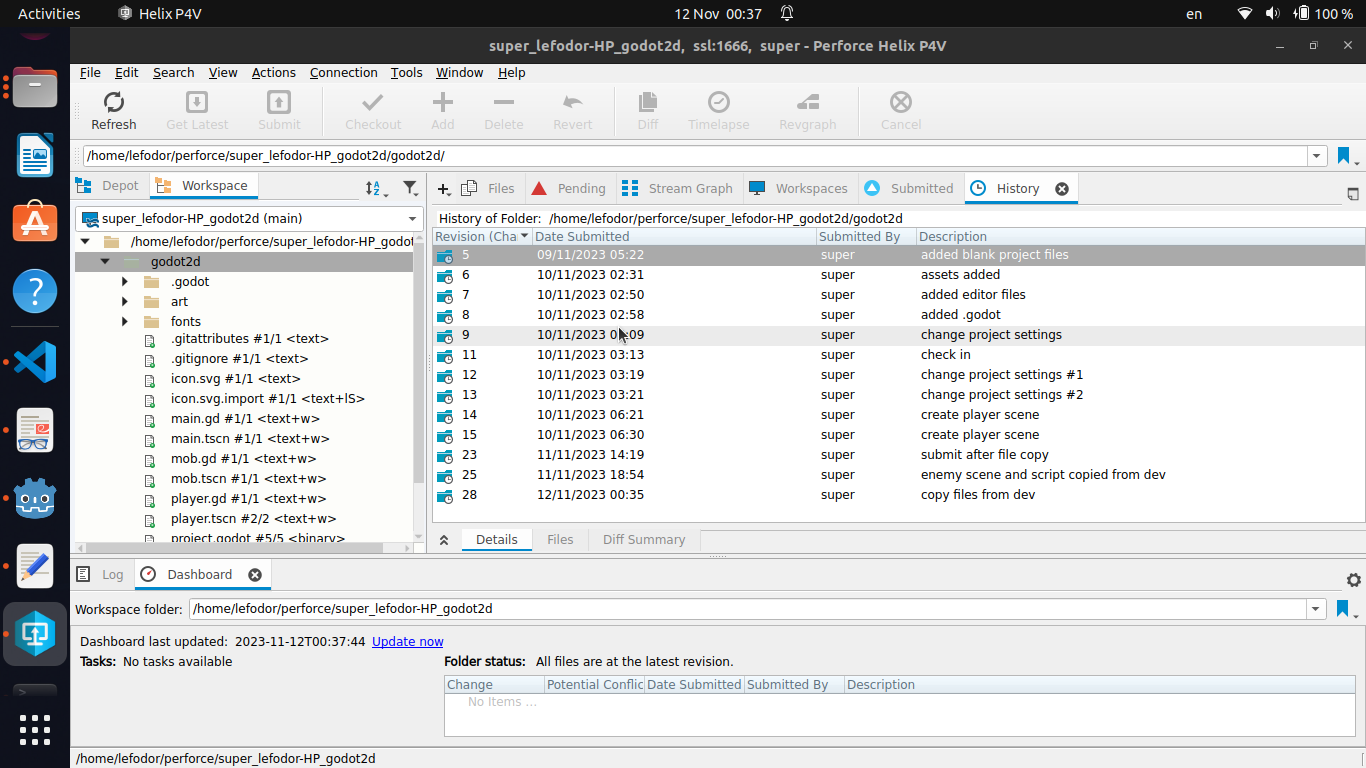
\includegraphics[width=\textwidth]{final-main-history.png}
    \caption{final main history}
    \label{fig:final-main-history}
\end{figure}